We are now ready to perform the experiments. We will begin exploring SimCLR implementation and results, later we will explore BYOL's implementation and lastly we will compare them in order to see how BYOL tries to improve SimCLR and we will check if it successess or not.

The code used for the experimentations, as well as some files with the results, can be found on the Github repository for this work.

\section{SimCLR exploration}
We will perform an iterative exploration with this framework. We will explore a few range for a subset of the hyperparameters and then we will go deeper into some hyperparameters to try and obtain better results.

\subsection{First approach}
\label{experiments:simclr:first}

The first thing we did to experiment with this framework is to explore a wide range of hyperparameters to see which set of them performed better for us. The script that can be found in \lstinline{code/SimCLR/run.py}.

What we did for this first exploration was to define a \emph{parameter grid} and execute the whole framework using each combination of the parameters. The parameters that were firstly considerered are:
\begin{enumerate}
\item \lstinline{batch_size}. This is one of the most important parameters of SimCLR. In the original paper, it was proven that the higher this parameter, the better the results obtained for the linear classification. This parameter is also important since it has to adapt to our GPU's memory. The options that we have considered for the first experiments are: \lstinline|batch_size = {512,1024}|.

\item \lstinline{temperature}. The temperature parameter $\tau$ plays an important role in the individual loss seen in Equation \eqref{c:loss:simclr:ind}. It is suggested to try values in the range $[0,1]$ and the one that had better performance for the original experiments was around $0.5$, so we chose the following values: \lstinline|temperature = {0.25,0.5,0.75,1}|.

\item \lstinline{color_jitter_strength}. This parameter measures how hard is the color variation in the data augmentation. Previous results show that this parameter is important for the success of the network, so we provide with a big range of values. We include the following values: \lstinline|color_jitter_strength = {0.25,0.5,0.75,1}|.
\end{enumerate}

Using python and the python function \lstinline{itertools.product} we straightforwardly generate all possible different combinations of unions of the parameters so we only have to append them to a general string and execute the \lstinline{run.py} script mentioned before to obtain the results. In total, we obtain $32$ possible combinations, so we will obtain $32$ models. 

The script was executed and took approximately $24$ hours to train and evaluate all the different models, obtaining the results in Table \ref{table:simclr:gridsearch:1} in Appendix \ref{APPENDIX:B}. We have to remark, for each of the two possible batch sizes, the best results obtained. These are:

\begin{table}[H]
    \label{table:best:first:simclr}
\centering
\resizebox{\columnwidth}{!}{
\begin{tabular}{rrrrrrr}
batch\_size   & temperature   & color\_jitter & regularization\_loss & top\_1\_accuracy & top\_5\_accuracy & steps         \\ \hline
 512  &  0.25 &  0.25 &  0.0093      &  0.833         &  0.994          &  9800 \\
 1024 &    0.25       &  0.75 &  0.0093      &  \textbf{0.841}          &  0.995          &  4900 \\
\end{tabular}
}
\caption{Best results for the grid search experiment with SimCLR.}
\end{table}

\begin{remark}
On the original paper, the Top 1 accuracy score reported for CIFAR10 in $100$ epochs was $\sim 84.6\%$ accuracy for batch size $512$ and $\sim 85.1 \%$ accuracy score for $1024$ batch size. If we have a look at the results obtained in our experiment, we can say that our first attempt was \emph{successfull}.
\end{remark}

Let us make some observations. The clearest is that, since the second batch size doubles the first one, the training ends in half the steps. We can see that the temperature obtained in both cases is the same, and it is equal to $0.25$. However, there is a big change in the color jitter parameter: while using $512$ as batch size obtains the best result with the value of $0.25$ for color jitter, using $1024$ as batch size this value changes to $0.75$, which implies stronger color changes on the data augmentation. 

In general, having a look again at the Table \ref{table:simclr:gridsearch:1} in Appendix \ref{APPENDIX:B},  we can see that:

\begin{itemize}
    \item As it also happens in the experiments made on the original SimCLR paper, lower temperature $\tau$ parameters cause higher accuracies on the linear heads of our models.
    
    \item The models perform better when the \lstinline{color_jitter} parameter is in the range $[0.5,0.75]$. This means that, in general, a generous amount of color jittering to our picture is benefitial for the models.

    \item The \emph{Top 5 accuracy} is above $99\%$ in each model. This says that, since the models almost always give the correct label one of the 5 highest values, but they obtain the correct tag around $84\%$ of the times, they might be creating some similar representations of the data for inputs that do not belong to the same class. 
\end{itemize}

\subsection*{Observations about the batch size}

Although both models get to the same value of regularization loss, the model with a batch size of $1024$ obtains a higher \emph{top 1 accuracy}. This seems to follow the intuitive idea that we presented before: SimCLR benefits from bigger batch sizes since it allows a positive sample to be compared and pushed appart from negative samples. Ideally, we would keep pushing the batch size parameter forward, doubling it again to try to find out if the performance of the model keeps benefiting from bigger batch sizes. However, this requires either using multiple GPUs(or TPUs) working in parallel on the training or using GPUs with bigger memory, which we do not have access to. 

Using the resources we have, the following experiment was performed: using the hyperparameters that we found out in our \emph{GridSearch} to be the ones that achieve the best results except for the \lstinline{batch-size}, we train models moving the batch size in the following range: 
$$
\text{\lstinline{batch-size}}=\{16,32,64,128,256,512,1024\},
$$
where the last two values had already been computed in the GridSearch so we do not have to repeat the training.

\begin{figure}[htp] 
    \centering
    \subfloat[Evolution of the Top 1 accuracy with the batch size.]{%
        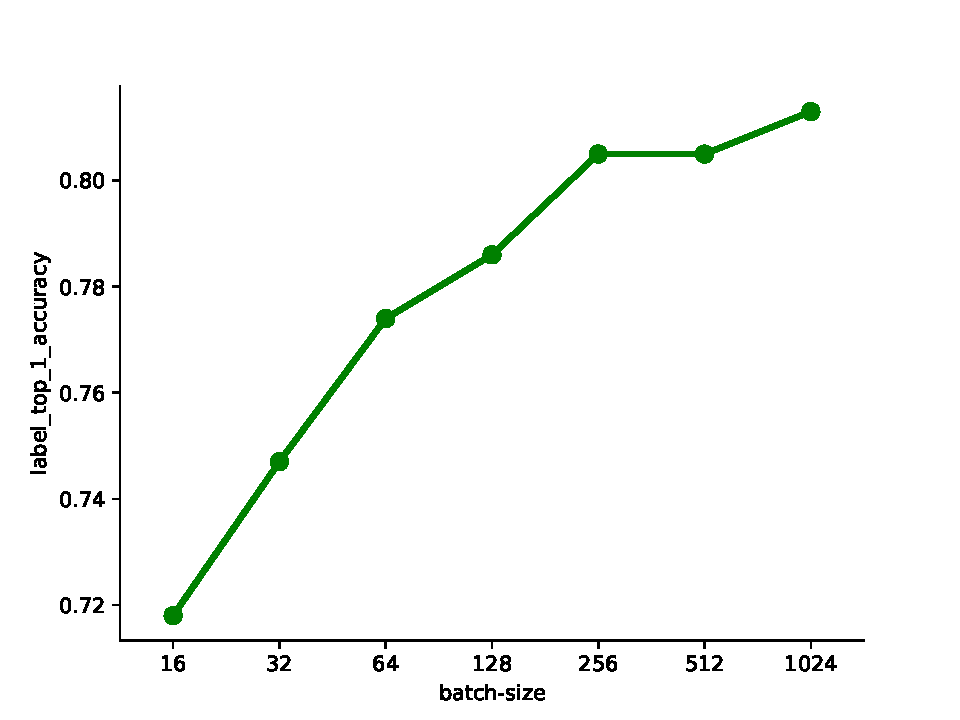
\includegraphics[width=0.45\textwidth]{simclr-batch-comparison}%
        \label{fig:accs:per:batch:simclr}%
        }%
    \hfill%
    \subfloat[Evolution curves of the accuracy with the steps taken in the training.]{%
        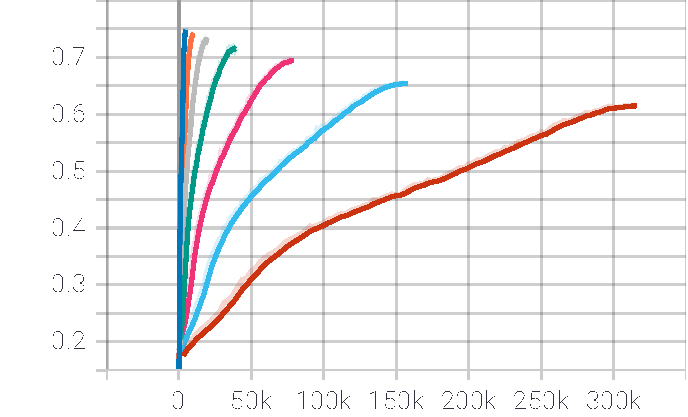
\includegraphics[width=0.45\textwidth]{train_supervised_acc}%
        \label{fig:evolution:acc:batches:simclr}%

        }%
        \caption{Results of the batch-size experiment.}
\end{figure}

Figure \ref{fig:accs:per:batch:simclr} shows the clear improvement of the Top 1 accuracy score when increasing the size of the batch that is used to compute the loss of our model. Increasing from $16$ to $1024$ gives an increase of more than $8\%$ in Top 1 accuracy, which is a lot. Further increase can be obtained if we keep increasing the batch size, but this is beyond our computation possibilities.

Figure \ref{fig:evolution:acc:batches:simclr} supports what we have just presented: not only with a smaller batch size we have to do thousands of extra steps in the training, but also we obtain much better accuracy performance of the linear head of the model.

\subsection*{Observations ofher hyperparameters}

We have seen that in our first experiment, batch size has been really relevant in the final results. We would like to see if the rest of the parameters play such an important role as well. 

As we have seen before, the parameters that we want to see how they affect the models are the \lstinline{color_jitter_strength} and the \lstinline{temperature} $\tau$ parameter. Let us study their impact on the model one by one. 

\begin{figure}[H] 
    \centering
    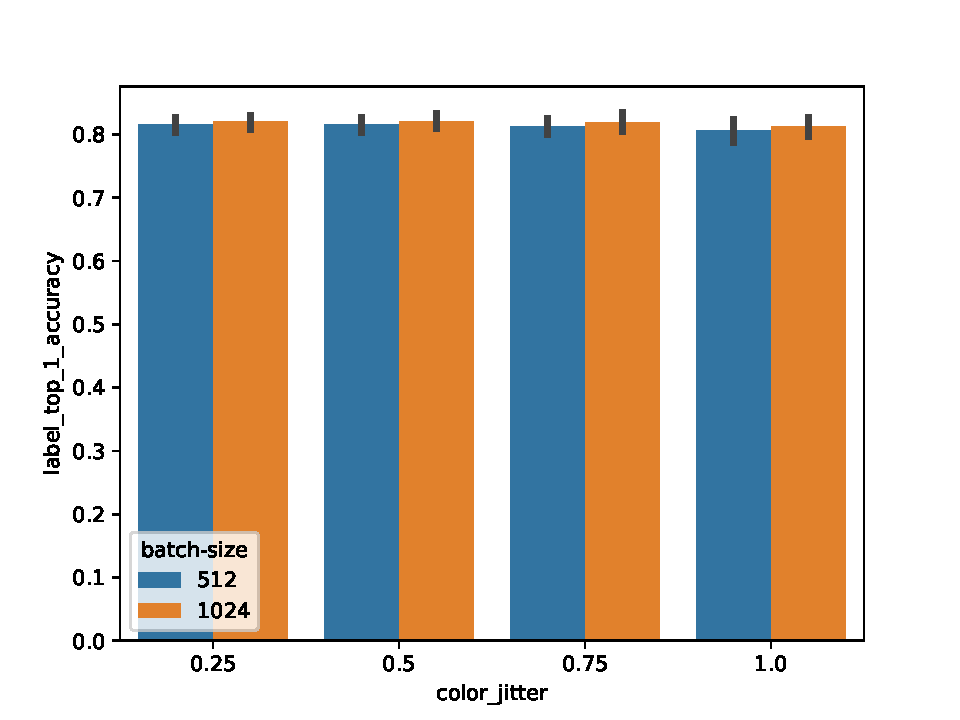
\includegraphics[width=0.55\textwidth]{color-jitter-impact-simclr}%
    
    \label{exp:simclr:colorjitter:impact}
    \caption{Acurracy score following the color jitter parameter and both batch sizes considered.}
\end{figure}

As we can see in Figure \ref{exp:simclr:colorjitter:impact}, the \lstinline{color_jitter_strength} parameter does not have a huge impact on the performance of the linear head of the model. The black bars on the center of each orange/blue bar indicate the variance of the accuracy respect the rest of the parameters. Surely, there are centesimal differences between the different values of this parameter. However, more finetuning might be needed in order to make this parameter relevant for our model. The low influence may as well be caused by the small encoder network (ResNet 18), so we will explore if there are any changes when we change the encoder network later in the document.

\begin{figure}[H] 
    \centering
    \label{exp:simclr:temperature:impact}
        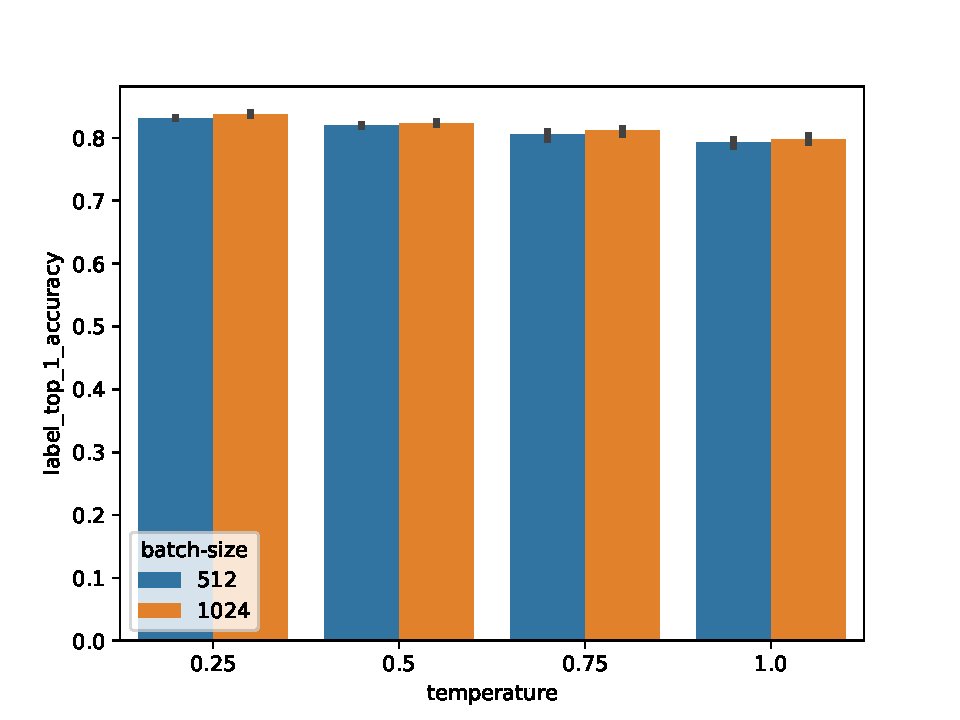
\includegraphics[width=0.55\textwidth]{temperature-impact-simclr}%
       
        \caption{Acurracy score following the temperature and both batch sizes considered.}
\end{figure}
